\section{Embedded Deployment Setup}
\label{sec:experimental_setup}

Deployment of machine learning models on microcontrollers while possible still poses some issues. MambaLite-Micro authors decided to pursue a path that would allow them to maintain exact same inference results as the trained PyTorch model, by extracting the weights from the model and hardcoding it in pure C. This approach, however, comes with many drawbacks, mainly that making any modifications to the model would need to also be implemented in C.

For this paper we decided not to go that route, and instead choose an already existing tool for porting a model to a microcontroller. There have been many different frameworks created, notably TensorFlow Lite Micro (now being renamed to LiteRT) \cite{davidTensorFlowLiteMicro2021} and ExecuTorch \cite{executorch2026}. We have investigated both of them and found that the hardware agnostic workflow of TFLM gives us more freedom for experimentation, has better documentation and causes less issues for deployment. This approach allows us to avoid many intermediary forms of the neural network (notably we do not convert the model to ONNX at any point). This eliminates the conversion differences between the interpretations from being a factor in the experiments.

Additionally there have been many tools built into and around TFLM. We are using the tflm\_model\_transforms, which strips all redundant and debug data from the model, which allows for fair comparison between model sizes by reducing the model graph overhead. We also use AI Edge Quantizer, which allows for precise control over the quantization process, and it operates directly on the tflite model files.

We also looked into other deployment options before deciding on the final one. The most interesting ones are Brevitas \cite{brevitas} (also used by FEMBA) and Torchao \cite{orTorchAOPyTorchNativeTrainingtoServing2025}. They both allow for quantization to be done on the PyTorch form of the model, and both of them allow for Quantization Aware Training, with the Brevitas additionally allowing for bit width quantization down to 1. In the final implementation we decided to not use them because of the need for kernel fusion that would arise after the QAT, which would be difficult to achieve efficiently for microcontrollers.

Because of time constraints of this project we also implemented and tested the models only on the ESP32 (\autoref{fig:esp32}) family of microcontrollers (ESP32, and ESP32S3). This was done using esp-tflite-micro, which is a vendor specific implementation of the TFLM. We decided against using a vendor specific deployment pipeline, such as ESP-DL or STM32Cube.AI, to make the results not be bound to only one MCU platform.

\begin{figure}
  \centering
  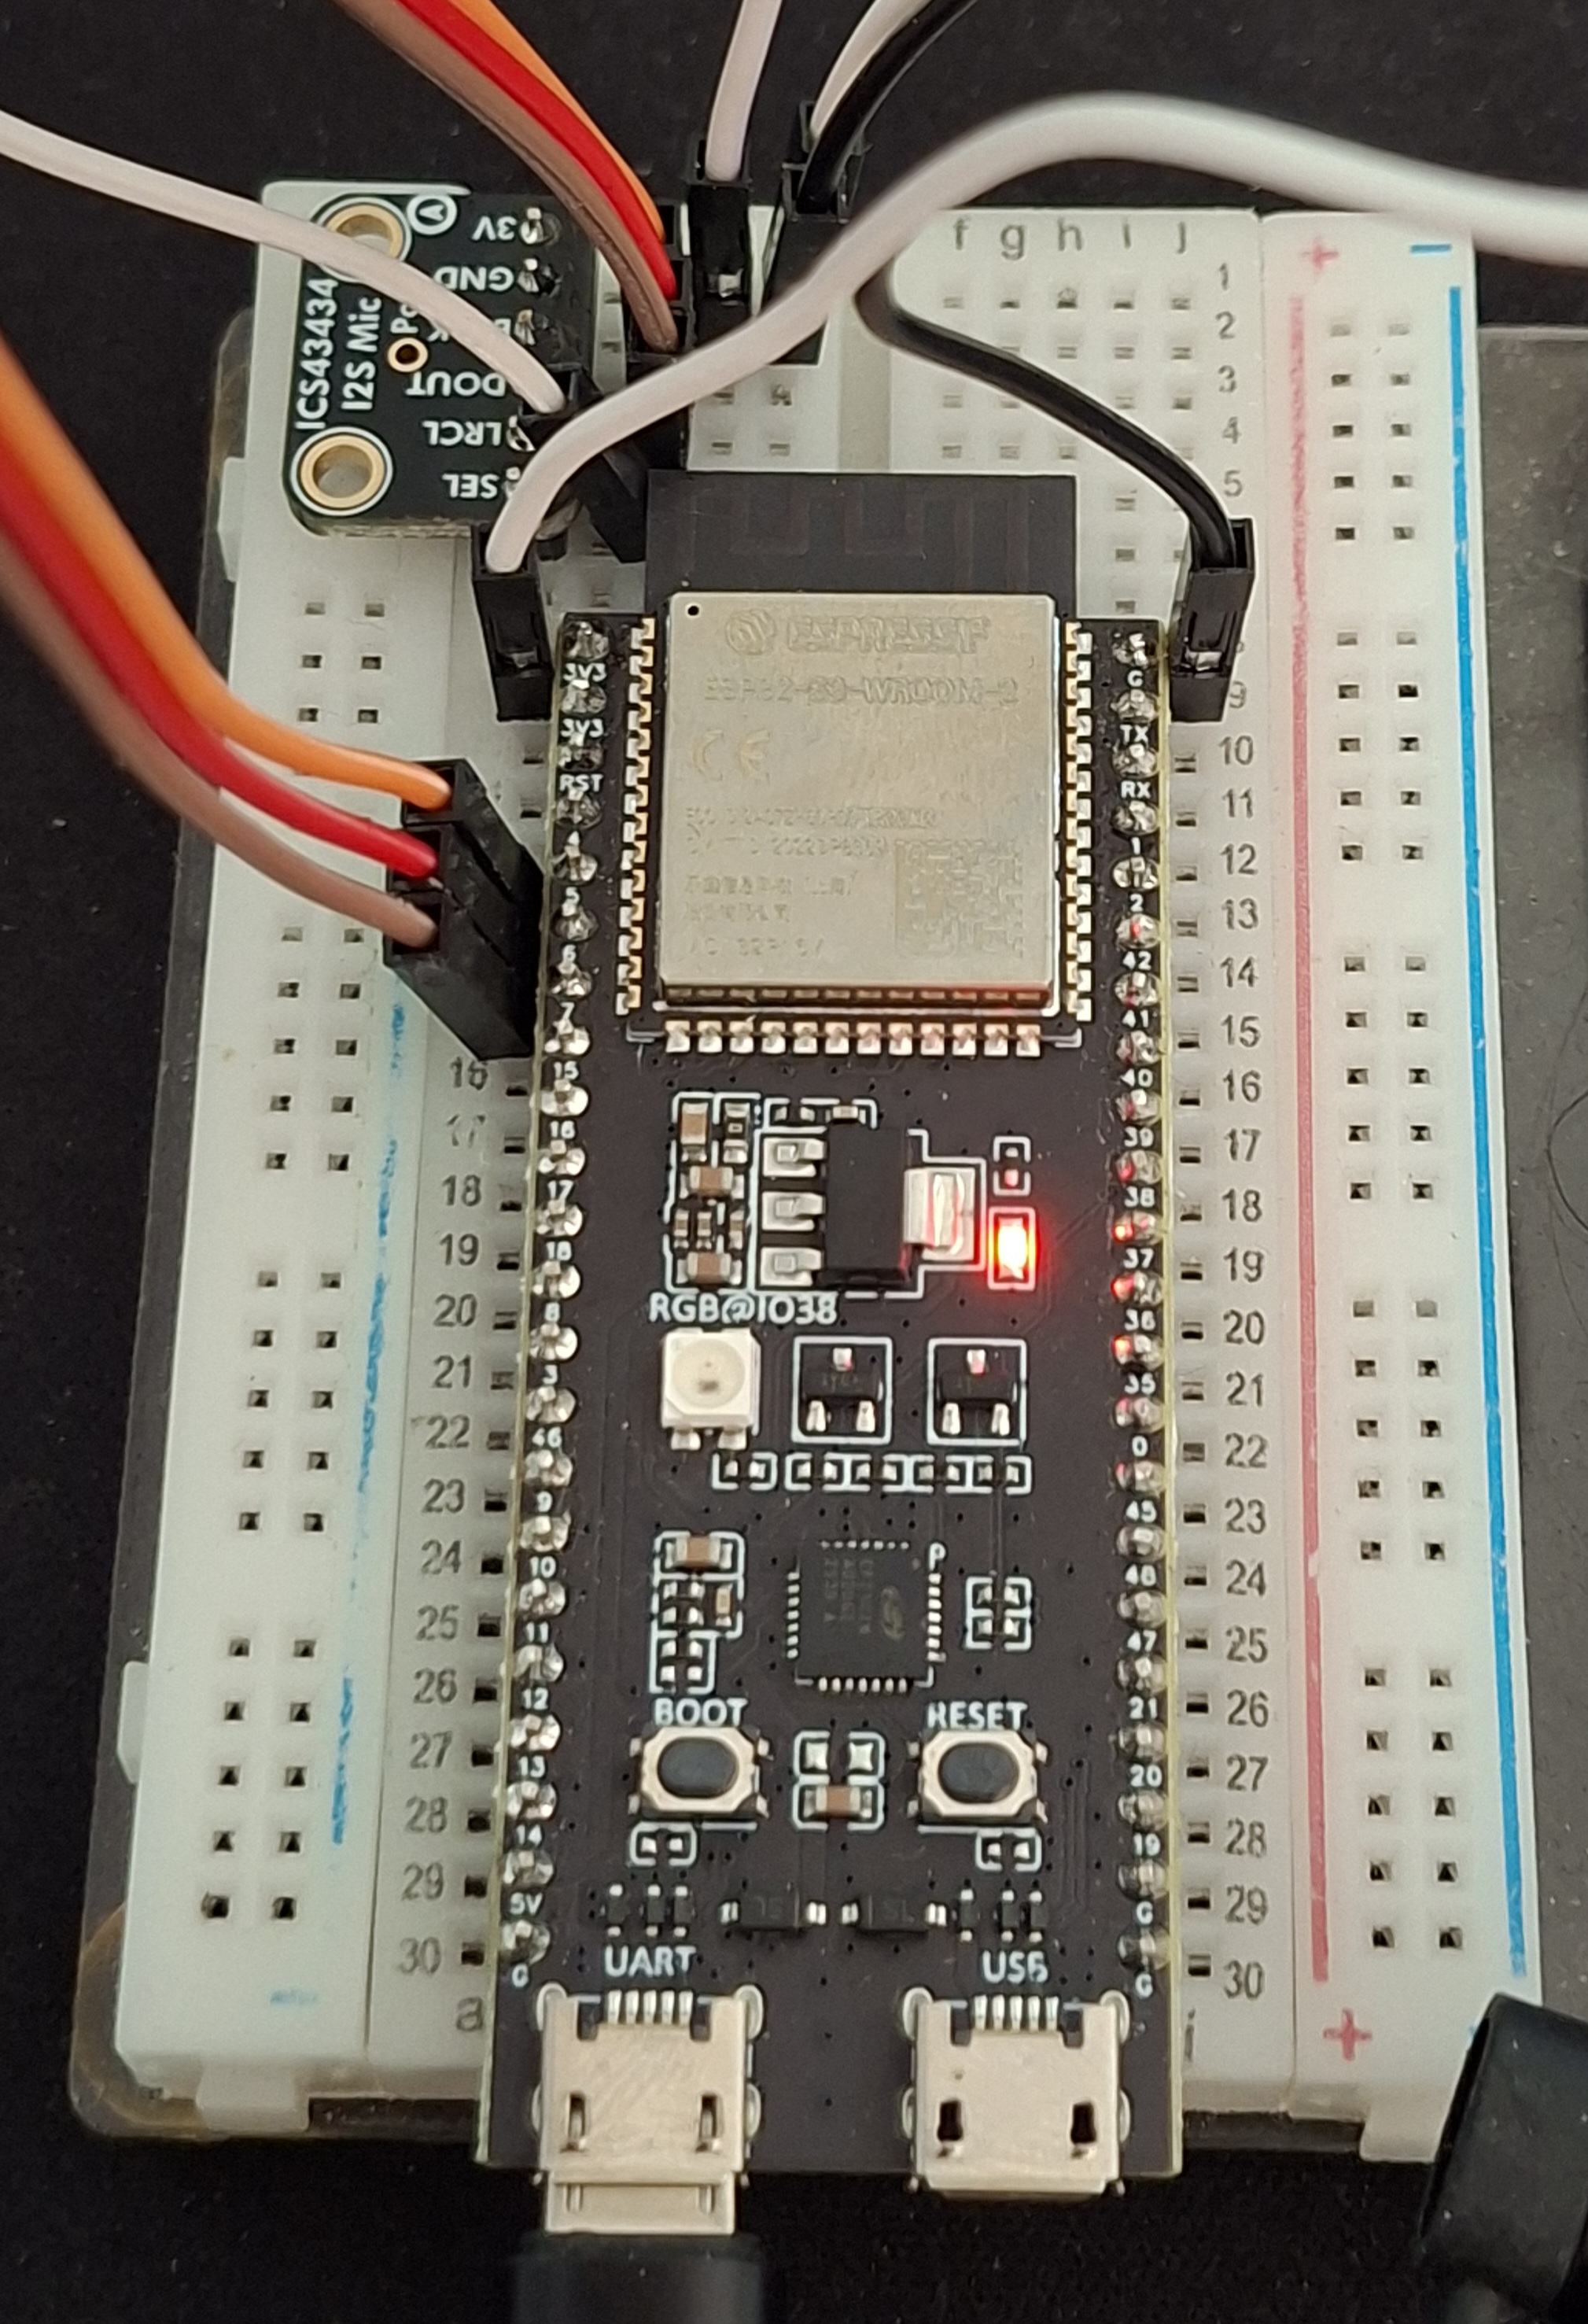
\includegraphics[width=0.5\linewidth]{assets/esp32.jpg}
  \caption{Photo of an ESP32S3 with ICS43434 microphone module attached}
  \label{fig:esp32}
\end{figure}
